\documentclass{beamer}
\usepackage{tikz,amsmath,hyperref,graphicx,stackrel,animate,tipa}
\usetikzlibrary{positioning,shadows,arrows,shapes,calc}
\newcommand{\ipa}[1]{\textipa{#1}}
\newcommand{\argmax}{\operatornamewithlimits{argmax}}
\newcommand{\argmin}{\operatornamewithlimits{argmin}}
\mode<presentation>{\usetheme{Frankfurt}}
\DeclareMathOperator*{\softmax}{softmax}
\AtBeginSection[]
{
  \begin{frame}<beamer>
    \frametitle{Outline}
    \tableofcontents[currentsection,currentsubsection]
  \end{frame}
}
\title{Hidden Markov Models}
\author{Mark Hasegawa-Johnson\\These slides are in the public domain}
\date{ECE 417: Multimedia Signal Processing}  
\begin{document}

% Title
\begin{frame}
  \maketitle
\end{frame}

% Title
\begin{frame}
  \tableofcontents
\end{frame}

%%%%%%%%%%%%%%%%%%%%%%%%%%%%%%%%%%%%%%%%%%%%
\section[HMM]{Hidden Markov Models}
\setcounter{subsection}{1}

\begin{frame}
  \frametitle{Notation: Inputs and Outputs}

  \begin{itemize}
  \item Let's assume we have $T$ consecutive 
    observations, $\mathbf{X}=[\mathbf{x}_1,\ldots,\mathbf{x}_T]$.
  \item A ``hidden Markov model'' represents those probabilities by
    assuming some sort of ``hidden'' state sequence,
    $\mathbf{q}=[q_1,\ldots,q_T]^T$, where $q_t$ is the hidden (unknown) state
    variable at time $t$.
  \end{itemize}
  The idea is, can we model these probabilities well enough to solve
  problems like:
  \begin{enumerate}
  \item {\bf Recognition:} What's $\Pr\{\mathbf{X}\}$ given the  model?
  \item {\bf Segmentation:} What state is the model in at time $t$?
  \item {\bf Training:} Can we learn a model to fit some data?
  \end{enumerate}
\end{frame}

\begin{frame}
  \frametitle{Notation: Inputs and Outputs}

  \centerline{\includegraphics[width=\textwidth]{hmm_aligned_spectrogram_three.png}}
\end{frame}

\begin{frame}
  \frametitle{HMM: Key Concepts}

  An HMM is a ``generative model,'' meaning that it models the joint
  probability $\Pr\{\mathbf{q},\mathbf{X}\}$ using a model of the way in which those data
  might have been generated.  An HMM pretends the following
  generative process:
  \begin{enumerate}
  \item Start in state $q_t=i$ with pmf $\pi_i=\Pr\{q_1=i\}$.
  \item Generate an observation, $\mathbf{x}$, with pdf $b_i(\mathbf{x})=\Pr\{\mathbf{x}|q_t=i\}$.
  \item Transition to a new state, $q_{t+1}=j$, according to pmf $a_{i,j}=\Pr\{q_{t+1}=j|q_t=i\}$.
  \item Repeat.
  \end{enumerate}
\end{frame}
\begin{frame}
  \frametitle{HMM: Finite State Diagram}

  \begin{center}
    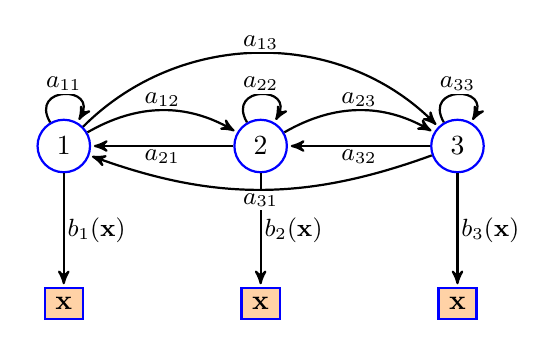
\begin{tikzpicture}[->,>=stealth',shorten >=1pt,auto,node distance=3cm,thick,
        state/.style={circle,thick,draw=blue,text=black,text centered,text width=0.25cm},
        obs/.style={rectangle,thick,draw=blue,text=black,fill=orange!35!white,text centered,text width=0.25cm}
      ]
      \node[state] (q1) at (0,0) {1};
      \node[state] (q2) at (2.5,0) {2};
      \node[state] (q3) at (5,0) {3};
      \node[obs] (x1) at (0,-2) {$\mathbf{x}$};
      \node[obs] (x2) at (2.5,-2) {$\mathbf{x}$};
      \node[obs] (x3) at (5,-2) {$\mathbf{x}$};
      \path[every node/.style={font=\sffamily\small,
  	  fill=white,inner sep=1pt}]
      (q1) edge [out=120,in=60,looseness=4] node {$a_{11}$} (q1)
      edge [out=30,in=150] node {$a_{12}$} (q2)
      edge [out=45,in=135] node {$a_{13}$} (q3)
      edge [out=-90,in=90] node {$b_1(\mathbf{x})$} (x1)
      (q2) edge [out=120,in=60,looseness=4] node {$a_{22}$} (q2)
      edge [out=180,in=0] node {$a_{21}$} (q1)
      edge [out=30,in=150] node {$a_{23}$} (q3)
      edge [out=-90,in=90] node {$b_2(\mathbf{x})$} (x2)
      (q3) edge [out=120,in=60,looseness=4] node {$a_{33}$} (q3)
      edge [out=180,in=0] node {$a_{32}$} (q2)
      edge [out=-160,in=-20] node {$a_{31}$} (q1)
      edge [out=-90,in=90] node {$b_3(\mathbf{x})$} (x3);
    \end{tikzpicture}
  \end{center}
  \begin{enumerate}
  \item Start in state $q_t=i$, for some $1\le i\le N$.
  \item Generate an observation, $\mathbf{x}$, with pdf $b_i(\mathbf{x})$.
  \item Transition to a new state, $q_{t+1}=j$, according to pmf $a_{i,j}$.
  \item Repeat steps \#2 and \#3, $T$ times each.
  \end{enumerate}
\end{frame}

\begin{frame}
  \frametitle{Notation: Model Parameters}

  Solving an HMM is possible if you {\bf carefully keep track of
  notation}.  Here's standard notation for the parameters:
  \begin{itemize}
  \item $\pi_i = \Pr\{q_1=i\}$ is called the {\bf initial state probability}.
    Let $N$ be the number of different states, so that $1\le i\le N$.
  \item $a_{i,j} = \Pr\{q_t=j|q_{t-1}=i\}$ is called the {\bf transition
    probability}, $1\le i,j\le N$.
  \item $b_j(\mathbf{x}) = \Pr\{\mathbf{x}_t=\mathbf{x}|q_t=j\}$ is called the
    {\bf observation probability}.  It is usually estimated by
    a neural network, though Gaussians, GMMs, and even lookup tables
    are possible.
  \item $\Lambda$ is the complete set of {\bf model parameters},
    including all the $\pi_i$'s and $a_{i,j}$'s, and the Gaussian, GMM,
    or neural net parameters necessary to compute $b_j(\mathbf{x})$.
  \end{itemize}
\end{frame}

\begin{frame}
  \frametitle{The Three Problems for an HMM}

  \begin{enumerate}
  \item {\bf Recognition:}
    \begin{itemize}
    \item Suppose our ASR knows two different words.  Each word is
      represented by a different set of model parameters: $\Lambda_1$
      and $\Lambda_2$.
    \item Suppose we have a test spectrogram, $\mathbf{X}$.  We know
      that $\mathbf{X}$ is one of those two words, but we don't know
      which.
    \item Which HMM was more likely to have produced $\mathbf{X}$?
      In other words, is
      $\Pr\{\mathbf{X}|\Lambda_1\}>\Pr\{\mathbf{X}|\Lambda_2\}$?
    \end{itemize}
  \item {\bf Segmentation:} What is $\Pr\{q_t=i|\mathbf{X},\Lambda\}$?
  \item {\bf Training:} Given an initial HMM $\Lambda$, and an
    observation sequence $\mathbf{X}$, can we find $\Lambda'$ such that
    $\Pr\{\mathbf{X}|\Lambda'\} > \Pr\{\mathbf{X}|\Lambda\}$?
  \end{enumerate}
\end{frame}

%%%%%%%%%%%%%%%%%%%%%%%%%%%%%%%%%%%%%%%%%%%%
\section[Recognition]{Recognition: the Forward Algorithm}
\setcounter{subsection}{1}

\begin{frame}
  \frametitle{The HMM Recognition Problem}

  \begin{itemize}
  \item Given \begin{itemize} \item $\mathbf{X} = [\mathbf{x}_1,\ldots,\mathbf{x}_T]$ and
    \item $\Lambda=\left\{\pi_i,a_{i,j},b_j(\mathbf{x})\forall i,j\right\}$,\end{itemize} what is $\Pr\{\mathbf{X}|\Lambda\}$?
  \item Let's solve a simpler problem first:
  \item Given \begin{itemize}\item $\mathbf{X} = [\mathbf{x}_1,\ldots,\mathbf{x}_T]$ and
    \item $\mathbf{q} = [q_1,\ldots,q_T]^T$ and
    \item $\Lambda=\left\{\pi_i,a_{i,j},b_j(\mathbf{x})\forall i,j\right\}$,\end{itemize} what is $\Pr\{\mathbf{X}|\Lambda\}$?
  \end{itemize}
\end{frame}
  
\begin{frame}
  \frametitle{Joint Probability of State Sequence and Observation Sequence}

  The joint probability of the state sequence and the observation
  sequence is calculated iteratively, from beginning to end:
  \begin{itemize}
  \item The probability that $q_1=q_1$ is $\pi_{q_1}$.
  \item Given $q_1$, the probability of $\mathbf{x}_1$ is $b_{q_1}(\mathbf{x}_1)$.
  \item Given $q_1$, the probability of $q_2$ is $a_{q_1q_2}$.
  \item \ldots and so on\ldots
  \end{itemize}
  \[
  \Pr\{\mathbf{q},\mathbf{X}|\Lambda\}=\pi_{q_1}b_{q_1}(\mathbf{x}_1)\prod_{t=2}^T a_{q_{t-1}q_t}b_{q_t}(\mathbf{x}_t)
  \]
\end{frame}

\begin{frame}
  \frametitle{Probability of the Observation Sequence}

  The probability of the observation sequence, alone, is somewhat
  harder, because we have to solve this sum:
  \begin{align*}
    \Pr\{\mathbf{X}|\Lambda\} &= \sum_{\mathbf{q}} \Pr\{\mathbf{q},\mathbf{X}|\Lambda\}\\
    &= \sum_{q_T=1}^N\cdots\sum_{q_1=1}^N \Pr\{\mathbf{q},\mathbf{X}|\Lambda\}
  \end{align*}

  On the face of it, this calculation seems to have complexity
  ${\mathcal O}\left\{N^T\right\}$.  So for a very small 100-frame
  utterance, with only 10 states, we have a complexity of ${\mathcal
    O}\left\{10^{100}\right\}=$one google.
\end{frame}

\begin{frame}
  \frametitle{The Forward Algorithm}

  The solution is to use a kind of dynamic programming algorithm,
  called ``the forward algorithm.''  The forward probability is
  defined as follows:
  \[
  \alpha_t(i) \equiv \Pr\{\mathbf{x}_1,\ldots,\mathbf{x}_t,q_t=i|\Lambda\}
  \]
  Obviously, if we can find $\alpha_t(i)$ for all $i$ and all $t$, we
  will have solved the recognition problem, because
  \begin{align*}
    \Pr\{\mathbf{X}|\Lambda\} &= \Pr\{\mathbf{x}_1,\ldots,\mathbf{x}_T|\Lambda\}\\
    &= \sum_{i=1}^N \Pr\{\mathbf{x}_1,\ldots,\mathbf{x}_T,q_T=i|\Lambda\}\\
    &= \sum_{i=1}^N \alpha_T(i)
  \end{align*}
\end{frame}
  
\begin{frame}
  \frametitle{The Forward Algorithm}

  So, working with the definition $\alpha_t(i) \equiv
  \Pr\{\mathbf{x}_1,\ldots,\mathbf{x}_t,q_t=i|\Lambda\}$, let's see how we can
  actually calculate $\alpha_t(i)$.
  \begin{enumerate}
  \item {\bf Initialize:}
    \begin{align*}
      \alpha_1(i) &= \Pr\{q_1=i,\mathbf{x}_1|\Lambda\}\\
      &= \Pr\{q_1=i|\Lambda\}\Pr\{\mathbf{x}_1|q_1=i,\Lambda\}\\
      &= \pi_i b_i(\mathbf{x}_1)
    \end{align*}
  \end{enumerate}
\end{frame}
  
\begin{frame}
  \frametitle{The Forward Algorithm}

  Definition: $\alpha_t(i) \equiv \Pr\{\mathbf{x}_1,\ldots,\mathbf{x}_t,q_t=i|\Lambda\}$.
  \begin{enumerate}
  \item {\bf Initialize:}
    \[
    \alpha_1(i) = \pi_i b_i(\mathbf{x}_1),~~~1\le i\le N
    \]
  \item {\bf Iterate:}
  \end{enumerate}
  \begin{align*}
    \alpha_{t}(j) &= \Pr\{\mathbf{x}_1,\ldots,\mathbf{x}_t,q_t=j|\Lambda\}\\
    &= \sum_{i=1}^N \Pr\{\mathbf{x}_1,\ldots,\mathbf{x}_{t-1},q_{t-1}=i\}\Pr\{q_t=j|q_{t-1}=i\}\Pr\{\mathbf{x}_t|q_t=j\}\\
    &= \sum_{i=1}^N \alpha_{t-1}(i) a_{i,j}b_j(\mathbf{x}_t)
  \end{align*}
\end{frame}
  
\begin{frame}
  \frametitle{The Forward Algorithm}

  So, working with the definition $\alpha_t(i) \equiv
  \Pr\{\mathbf{x}_1,\ldots,\mathbf{x}_t,q_t=i|\Lambda\}$, let's see how we can
  actually calculate $\alpha_t(i)$.
  \begin{enumerate}
  \item {\bf Initialize:}
    \[
    \alpha_1(i) = \pi_i b_i(\mathbf{x}_1),~~~1\le i\le N
    \]
  \item {\bf Iterate:}
    \begin{align*}
      \alpha_{t}(j) &= \sum_{i=1}^N \alpha_{t-1}(i) a_{i,j}b_j(\mathbf{x}_t),~~1\le j\le N,~2\le t\le T
    \end{align*}
  \item {\bf Terminate:}
    \[
    \Pr\{\mathbf{X}|\Lambda\} = \sum_{i=1}^N \alpha_T(i)
    \]
  \end{enumerate}
\end{frame}

\begin{frame}
  \frametitle{Visualizing the Forward Algorithm using a Trellis}

  One way to think about the forward algorithm is by way of a {\bf
    trellis}.  A trellis is a matrix in which each time step is a
  column, and each row shows a different state.  For example, here's a
  trellis with $N=4$ states, and $T=5$ frames:
  
  \centerline{\includegraphics[width=\textwidth]{exp/640px-Convolutional_code_trellis_diagram.svg.png}}
  \centerline{\small Public domain image by Qef, 2009}
\end{frame}

\begin{frame}
  \frametitle{Visualizing the Forward Algorithm using a Trellis}

  \centerline{\includegraphics[width=\textwidth]{exp/640px-Convolutional_code_trellis_diagram.svg.png}}

  Using a trellis, the {\bf initialize} step computes probabilities
  for the first column of the trellis:
  \[
  \alpha_1(i) = \pi_i b_i(\mathbf{x}_1),~~~1\le i\le N
  \]  
\end{frame}

\begin{frame}
  \frametitle{Visualizing the Forward Algorithm using a Trellis}

  \centerline{\includegraphics[width=\textwidth]{exp/640px-Convolutional_code_trellis_diagram.svg.png}}

  The {\bf iterate} step then computes the probabilities in the
  $t^{\textrm{th}}$ column by adding up the probabilities in the
  $(t-1)^{\textrm{st}}$ column, each multiplied by the corresponding
  transition probability:
  \begin{align*}
    \alpha_{t}(j) &= \sum_{i=1}^N \alpha_{t-1}(i) a_{i,j}b_j(\mathbf{x}_t),~~1\le j\le N,~2\le t\le T
  \end{align*}
\end{frame}

\begin{frame}
  \frametitle{Visualizing the Forward Algorithm using a Trellis}

  \centerline{\includegraphics[width=\textwidth]{exp/640px-Convolutional_code_trellis_diagram.svg.png}}

  The {\bf terminate} step then computes the likelihood of the model
  by adding the probabilities in the last column:
  \[
  \Pr\{\mathbf{X}|\Lambda\} = \sum_{i=1}^N \alpha_T(i)
  \]
\end{frame}
  
\begin{frame}
  \frametitle{The Forward Algorithm: Computational Complexity}

  Most of the computational complexity is in this step:
  \begin{itemize}
  \item {\bf Iterate:}
    \[
    \alpha_{t}(j) = \sum_{i=1}^N \alpha_{t-1}(i) a_{i,j}b_j(\mathbf{x}_t),~~1\le i,j\le N,~2\le t\le T
    \]
  \end{itemize}
  Its complexity is:
  \begin{itemize}
  \item For each of $T-1$ time steps, $2\le t\le T$,\ldots
  \item we need to calculate $N$ different alpha-variables, $\alpha_t(j)$, for $1\le j\le N$,\ldots
  \item each of which requires a summation with $N$ terms.
  \end{itemize}
  So the total complexity is ${\mathcal O}\left\{TN^2\right\}$.  For
  example, with $N=10$ and $T=100$, the complexity is only $TN^2=10,000$
  multiplies (much, much less than $N^T$!!)
\end{frame}

%%%%%%%%%%%%%%%%%%%%%%%%%%%%%%%%%%%%%%%%%%%%
\section[Segmentation]{Segmentation: the Backward Algorithm}
\setcounter{subsection}{1}

\begin{frame}
  \frametitle{The Segmentation Problem}

  There are different ways to define the segmentation problem.  Let's
  define it this way:
  \begin{itemize}
  \item We want to find the most likely state, $q_t=i$, at time $t$,\ldots
  \item given knowledge of the {\em entire} sequence
    $\mathbf{X}=[\mathbf{x}_1,\ldots,\mathbf{x}_T]$, not just the current observation.
    So for example, we don't want to recognize state $i$ at time $t$ if
    the surrounding observations, $\mathbf{x}_{t-1}$ and $\mathbf{x}_{t+1}$, make it obvious that
    this choice is impossible.  Also,\ldots
  \item given knowledge of the HMM that produced this sequence, $\Lambda$.
  \end{itemize}

  In other words, we want to find the {\bf state posterior
    probability}, $\Pr\{q_t=i|\mathbf{X},\Lambda\}$.  Let's define some more
  notation for the state posterior probability, let's call it
  \[
  \gamma_t(i) = \Pr\{q_t=i|\mathbf{X},\Lambda\}
  \]
\end{frame}

\begin{frame}
  \frametitle{Use Bayes' Rule}

  Suppose we already knew the {\bf joint probability,}
  $\Pr\{\mathbf{X},q_t=i|\Lambda\}$.  Then we could find the state posterior using
  Bayes' rule:
  \begin{displaymath}
    \gamma_t(i) = \Pr\{q_t=i|\mathbf{X},\Lambda\} = \frac{\Pr\{\mathbf{X},q_t=i|\Lambda\}}{\sum_{j=1}^N \Pr\{\mathbf{X},q_t=j|\Lambda\}}
  \end{displaymath}
\end{frame}

\begin{frame}
  \frametitle{Use the Forward Algorithm}

  Let's expand this:
  \[
  \Pr\{\mathbf{X},q_t=i|\Lambda\} = \Pr\{q_t=i,\mathbf{x}_1,\ldots,\mathbf{x}_T|\Lambda\}
  \]
  We already know about half of that: $\alpha_t(i)=\Pr\{q_t=i,\mathbf{x}_1,\ldots,\mathbf{x}_t|\Lambda\}$.
  We're only missing this part:
  \[
  \Pr\{\mathbf{X},q_t=i|\Lambda\} = \alpha_t(i)\Pr\{\mathbf{x}_{t+1},\ldots,\mathbf{x}_T|q_t=i,\Lambda\}
  \]
  Again, let's try the trick of ``solve the problem by inventing new notation.''  Let's define
  \[
  \beta_t(i) \equiv \Pr\{\mathbf{x}_{t+1},\ldots,\mathbf{x}_T|q_t=i,\Lambda\}
  \]
\end{frame}

\begin{frame}
  \frametitle{The Backward Algorithm}

  Now let's use the definition
  $\beta_t(i)\equiv \Pr\{\mathbf{x}_{t+1},\ldots,\mathbf{x}_T|q_t=i,\Lambda\}$, and see how we can
  compute that.
  \begin{enumerate}
  \item {\bf Initialize:}
    \[
    \beta_T(i) = 1,~~1\le i\le N
    \]
    This might not seem immediately obvious, but think about it.
    Given that there are no more $\mathbf{x}$ vectors after time $T$,
    what is the probability that there are no more $\mathbf{x}$ vectors
    after time $T$?  Well, 1, obviously.
  \end{enumerate}
\end{frame}

\begin{frame}
  \frametitle{The Backward Algorithm}

  Now let's use the definition $\beta_t(i) \equiv
  \Pr\{\mathbf{x}_{t+1},\ldots,\mathbf{x}_T|q_t=i,\Lambda\}$, and see how we can
  compute that.
  \begin{enumerate}
  \item {\bf Initialize:}
    \[
    \beta_T(i) = 1,~~1\le i\le N
    \]
  \item {\bf Iterate:}
  \end{enumerate}
  \begin{align*}
    &\beta_{t}(i) = \Pr\{\mathbf{x}_{t+1},\ldots,\mathbf{x}_T|q_t=i,\Lambda\}\\
    &= \sum_{j=1}^N \Pr\{q_{t+1}=j|q_t=i\}\Pr\{\mathbf{x}_{t+1}|q_{t+1}=j\}\Pr\{\mathbf{x}_{t+2},\ldots,\mathbf{x}_T|q_{t+1}=j\}\\
    &= \sum_{j=1}^N a_{i,j}b_j(\mathbf{x}_{t+1})\beta_{t+1}(j)
  \end{align*}
\end{frame}

\begin{frame}
  \frametitle{The Backward Algorithm}

  Now let's use the definition $\beta_t(i) \equiv
  \Pr\{\mathbf{x}_{t+1},\ldots,\mathbf{x}_T|q_t=i,\Lambda\}$, and see how we can
  compute that.
  \begin{enumerate}
  \item {\bf Initialize:}
    \[
    \beta_T(i) = 1,~~1\le i\le N
    \]
  \item {\bf Iterate:}
    \begin{align*}
      \beta_{t}(i) &= \sum_{j=1}^N a_{i,j}b_j(\mathbf{x}_{t+1})\beta_{t+1}(j),~~1\le i\le N,~1\le t\le T-1
    \end{align*}
  \item {\bf Terminate:}
    \[
    \Pr\{\mathbf{X}|\Lambda\} = \sum_{i=1}^N \pi_ib_i(\mathbf{x}_1)\beta_1(i)
    \]
  \end{enumerate}
\end{frame}

  
\begin{frame}
  \frametitle{The Backward Algorithm: Computational Complexity}

  Most of the computational complexity is in this step:
  \begin{itemize}
  \item {\bf Iterate:}
    \begin{align*}
      \beta_{t}(i) 
      &= \sum_{j=1}^N a_{i,j}b_j(\mathbf{x}_{t+1})\beta_{t+1}(j),~~1\le i\le N,~2\le t\le T
    \end{align*}
  \end{itemize}
  Its complexity is:
  \begin{itemize}
  \item For each of $T-1$ time steps, $1\le t\le T-1$,\ldots
  \item we need to calculate $N$ different beta-variables, $\beta_t(i)$, for $1\le i\le N$,\ldots
  \item each of which requires a summation with $N$ terms.
  \end{itemize}
  So the total complexity is ${\mathcal O}\left\{TN^2\right\}$.
\end{frame}

\begin{frame}
  \frametitle{Use Bayes' Rule}

  The segmentation probability is then
  \begin{align*}
    \gamma_t(i) &= \frac{\Pr\{X,q_t=i|\Lambda\}}{\sum_{k=1}^N \Pr\{\mathbf{X},q_t=k|\Lambda\}}\\
    &= \frac{\Pr\{\mathbf{x}_1,\ldots,\mathbf{x}_t,q_t=i|\Lambda\}\Pr\{\mathbf{x}_{t+1},\ldots,\mathbf{x}_T|q_t=i,\Lambda\}}{\sum_{k=1}^N \Pr\{\mathbf{x}_1,\ldots,\mathbf{x}_t,q_t=k|\Lambda\}\Pr\{\mathbf{x}_{t+1},\ldots,\mathbf{x}_T|q_t=k,\Lambda\}}\\
    &= \frac{\alpha_t(i)\beta_t(i)}{\sum_{k=1}^N\alpha_t(k)\beta_t(k)}
  \end{align*}
\end{frame}

\begin{frame}
  \frametitle{What About State Sequences?}

  \begin{itemize}
  \item Notice a problem: $\gamma_t(i)$ only tells us about one frame at a time!  It doesn't tell
    us anything about the probability of a sequence of states, covering a sequence of frames!
  \item \ldots but we can extend the same reasoning to cover two or
    more consecutive frames.  For example, let's define:
    \[
    \xi_t(i,j) = \Pr\{q_t=i,q_{t+1}=j|\mathbf{X},\Lambda\}
    \]
    \item We can solve for $\xi_t(i,j)$ using the same reasoning that
      we used for $\gamma_t(i)$!  The result is
      \begin{displaymath}
        \xi_t(i,j)=\frac{\alpha_t(i)a_{i,j}b_{j}(\mathbf{x}_{t+1})\beta_{t=1}(j)}{\sum_{k=1}^N\sum_{\ell=1}^N\alpha_t(k)a_{k,\ell}b_{\ell}(\mathbf{x}_{t+1})\beta_{t=1}(\ell)}
      \end{displaymath}
  \end{itemize}
\end{frame}

\begin{frame}
  \frametitle{Segmentation: The Backward Algorithm}

  In summary, we now have three new probabilities, all of which can be
  computed in ${\mathcal O}\left\{TN^2\right\}$ time:
  \begin{enumerate}
  \item {\bf The Backward Probability:}
    \[
    \beta_t(i) = \Pr\{\mathbf{x}_{t+1},\ldots,\mathbf{x}_T|q_t=i,\Lambda\}
    \]
  \item {\bf The State Posterior:}
    \begin{align*}
      \gamma_t(i) & = \Pr\{q_t=i|X,\Lambda\}
      = \frac{\alpha_t(i)\beta_t(i)}{\sum_{k=1}^N\alpha_t(k)\beta_t(k)}
    \end{align*}
  \item {\bf The Segment Posterior:}
    \begin{align*}
      \xi_t(i,j) & = \Pr\{q_t=i,q_{t+1}=j|X,\Lambda\}\\
      &= \frac{\alpha_t(i)a_{i,j}b_j(\mathbf{x}_{t+1})\beta_{t+1}(j)}{\sum_{k=1}^N\sum_{\ell=1}^N\alpha_t(k)a_{k\ell}b_\ell(\mathbf{x}_{t+1})\beta_{t+1}(\ell)}
    \end{align*}
  \end{enumerate}
\end{frame}

%%%%%%%%%%%%%%%%%%%%%%%%%%%%%%%%%%%%%%%%%%%%
\section[Example]{Numerical Example}
\setcounter{subsection}{1}

\begin{frame}
  \frametitle{Example: Gumball Machines}
  \centerline{\includegraphics[height=2.5in]{exp/Gumball_machines_Dallas_2008.jpg}}
  \begin{tiny}
    ``Gumball machines in a Diner at Dallas, Texas, in 2008,'' Andreas Praefcke, public domain image.
  \end{tiny}
\end{frame}

\begin{frame}
  \frametitle{Example: Gumball Machines}
  \begin{itemize}
  \item {\bf Observation Probabilities:} Suppose we have two gumball
    machines, $q=1$ and $q=2$.  Machine \#1 contains 60\% Grapefruit
    gumballs, 40\% Apple gumballs.  Machine \#2 contains 90\%
    Apple, 10\% Grapefruit.
    \[
    b_1(x)=\begin{cases} 0.4 & x=A\\0.6 & x=G\end{cases},~~~
    b_2(x)=\begin{cases} 0.9 & x=A\\0.1 & x=G\end{cases}
    \]
  \item {\bf Initial State Probabilities:} My friend George flips a
    coin to decide which machine to use first.
    \[
    \pi_i = 0.5,~~~i\in\left\{1,2\right\}
    \]
  \item {\bf Transition Probabilities:} After he's used a machine,
    George flips two coins, and he only changes machines if both coins
    come up heads.
    \[
    a_{i,j}=\begin{cases} 0.75 & i=j\\0.25 & i\ne j\end{cases}
    \]
  \end{itemize}
\end{frame}

\begin{frame}
  \frametitle{A Segmentation Problem}

  \begin{itemize}
  \item George bought three gumballs, using three quarters.  The three
    gumballs are $(x_1=A,x_2=G,x_3=A)$.
  \item Unfortunately, George is a bit of a goofball.  The second of
    the three ``quarters'' was actually my 1867 silver ``Seated
    Liberty'' dollar, worth \$4467.
  \item Which of the two machines do I need to dismantle in order to
    get my coin back?
  \end{itemize}
  \centerline{\includegraphics[height=1in]{exp/seatedlibertydollar.jpg}}
  \begin{tiny}Image used with permission of the National Numismatic Collection, National Museum of American History.\end{tiny}
\end{frame}

\begin{frame}
  \frametitle{The Forward Algorithm: $t=1$}

  Remember, the observation sequence is $X=(A,G,A)$.
  \begin{align*}
  \alpha_1(i) &= \pi_i b_1(i) \\
  &= \begin{cases} (0.5)(0.4)=0.2  & i=1\\(0.5)(0.9)=0.45 & i=2\end{cases}
  \end{align*}
\end{frame}

\begin{frame}
  \frametitle{The Forward Algorithm: $t=2$}

  Remember, the observation sequence is $X=(A,G,A)$.
  \begin{align*}
  \alpha_2(j) &= \sum_{i=1}^2 \alpha_1(i)a_{i,j}b_j(x_2)\\
  &= \begin{cases}
    \alpha_1(1)a_{11}b_1(x_2)+\alpha_1(2)a_{21}b_1(x_2) & j=1\\
    \alpha_1(1)a_{12}b_2(x_2)+\alpha_1(2)a_{22}b_2(x_2) & j=2
  \end{cases}\\
  &= \begin{cases}
    (0.2)(0.75)(0.6)+(0.45)(0.25)(0.6)=0.04125  & j=1\\
    (0.2)(0.25)(0.1)+(0.45)(0.75)(0.1)=0.03875 &  j=2
  \end{cases}
  \end{align*}
  
\end{frame}

\begin{frame}
  \frametitle{The Backward Algorithm: $t=3$}

  The backward algorithm always starts out with $\beta_T(i)=1$! 
  \begin{align*}
  \beta_3(i) &= 1,~~~i\in\left\{1,2\right\}
  \end{align*}
  
\end{frame}

\begin{frame}
  \frametitle{The Backward Algorithm: $t=2$}

  Remember, the observation sequence is $X=(A,G,A)$.
  \begin{align*}
  \beta_2(i) &= \sum_{j=1}^2 a_{i,j}b_j(x_3)\beta_3(j)\\
  &= \begin{cases}
    a_{11}b_1(x_3)+a_{12}b_2(x_3) & i=1\\
    a_{21}b_1(x_3)+a_{22}b_2(x_3) & i=2
  \end{cases}\\
  &= \begin{cases}
    (0.75)(0.4)+(0.25)(0.9)=0.525 & j=1\\
    (0.25)(0.4)+(0.75)(0.9)=0.775 & j=2
  \end{cases}
  \end{align*}  
\end{frame}

\begin{frame}
  \frametitle{The Solution to the Puzzle}

  Given the observation sequence is $X=(A,G,A)$, 
  the posterior state probability is
  \begin{align*}
    \gamma_2(i)&=\frac{\alpha_2(i)\beta_2(i)}{\sum_{k=1}^2\alpha_2(k)\beta_2(k)}\\
    &= \begin{cases}
      \frac{(0.04125)(0.525)}{(0.04125)(0.525)+(0.03875)(0.775)}
      = 0.42 & i=1\\
      \frac{(0.03875)(0.775)}{(0.04125)(0.525)+(0.03875)(0.775)}
      = 0.58 & i=2
    \end{cases}
  \end{align*}
  So I should dismantle gumball machine \#2, hoping to find my rare
  1867 silver dollar.  Good luck!
\end{frame}

%%%%%%%%%%%%%%%%%%%%%%%%%%%%%%%%%%%%%%%%%%%%
\section[Summary]{Summary}
\setcounter{subsection}{1}

\begin{frame}
  \frametitle{The Forward Algorithm}

  Definition: $\alpha_t(i) \equiv \Pr\{\mathbf{x}_1,\ldots,\mathbf{x}_t,q_t=i|\Lambda\}$.  Computation:
  \begin{enumerate}
  \item {\bf Initialize:}
    \[
    \alpha_1(i) = \pi_i b_i(\mathbf{x}_1),~~~1\le i\le N
    \]
  \item {\bf Iterate:}
    \begin{align*}
      \alpha_{t}(j) &= \sum_{i=1}^N \alpha_{t-1}(i) a_{i,j}b_j(\mathbf{x}_t),~~1\le j\le N,~2\le t\le T
    \end{align*}
  \item {\bf Terminate:}
    \[
    \Pr\{\mathbf{X}|\Lambda\} = \sum_{i=1}^N \alpha_T(i)
    \]
  \end{enumerate}
\end{frame}
  
\begin{frame}
  \frametitle{The Backward Algorithm}

  Definition: $\beta_t(i) \equiv \Pr\{\mathbf{x}_{t+1},\ldots,\mathbf{x}_T|q_t=i,\Lambda\}$.  Computation:
  \begin{enumerate}
  \item {\bf Initialize:}
    \[
    \beta_T(i) = 1,~~~1\le i\le N
    \]
  \item {\bf Iterate:}
    \begin{align*}
      \beta_{t}(i) &= \sum_{j=1}^N a_{i,j}b_j(\mathbf{x}_{t+1})\beta_{t+1}(j),~~1\le i\le N,~1\le t\le T-1
    \end{align*}
  \item {\bf Terminate:}
    \[
    \Pr\{\mathbf{X}|\Lambda\} = \sum_{i=1}^N \pi_ib_i(\mathbf{x}_1)\beta_1(i)
    \]
  \end{enumerate}
\end{frame}

\begin{frame}
  \frametitle{Hidden Markov Model}

  \begin{center}
    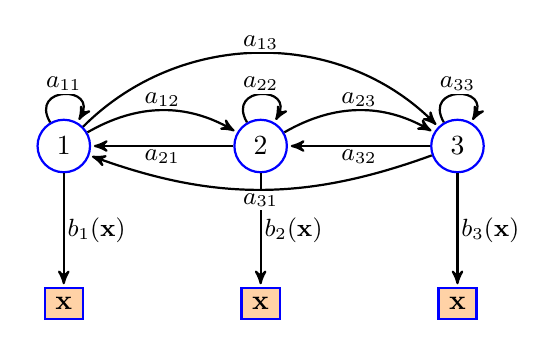
\begin{tikzpicture}[->,>=stealth',shorten >=1pt,auto,node distance=3cm,thick,
        state/.style={circle,thick,draw=blue,text=black,text centered,text width=0.25cm},
        obs/.style={rectangle,thick,draw=blue,text=black,fill=orange!35!white,text centered,text width=0.25cm}
      ]
      \node[state] (q1) at (0,0) {1};
      \node[state] (q2) at (2.5,0) {2};
      \node[state] (q3) at (5,0) {3};
      \node[obs] (x1) at (0,-2) {$\mathbf{x}$};
      \node[obs] (x2) at (2.5,-2) {$\mathbf{x}$};
      \node[obs] (x3) at (5,-2) {$\mathbf{x}$};
      \path[every node/.style={font=\sffamily\small,
  	  fill=white,inner sep=1pt}]
      (q1) edge [out=120,in=60,looseness=4] node {$a_{11}$} (q1)
      edge [out=30,in=150] node {$a_{12}$} (q2)
      edge [out=45,in=135] node {$a_{13}$} (q3)
      edge [out=-90,in=90] node {$b_1(\mathbf{x})$} (x1)
      (q2) edge [out=120,in=60,looseness=4] node {$a_{22}$} (q2)
      edge [out=180,in=0] node {$a_{21}$} (q1)
      edge [out=30,in=150] node {$a_{23}$} (q3)
      edge [out=-90,in=90] node {$b_2(\mathbf{x})$} (x2)
      (q3) edge [out=120,in=60,looseness=4] node {$a_{33}$} (q3)
      edge [out=180,in=0] node {$a_{32}$} (q2)
      edge [out=-160,in=-20] node {$a_{31}$} (q1)
      edge [out=-90,in=90] node {$b_3(\mathbf{x})$} (x3);
    \end{tikzpicture}
  \end{center}
  \begin{enumerate}
  \item Start in state $q_t=i$ with pmf $\pi_i$.
  \item Generate an observation, $\mathbf{x}$, with pdf $b_i(\mathbf{x})$.
  \item Transition to a new state, $q_{t+1}=j$, according to pmf $a_{i,j}$.
  \item Repeat.
  \end{enumerate}
\end{frame}

%%%%%%%%%%%%%%%%%%%%%%%%%%%%%%%%%%%%%%%%%%%%
\section[Example]{Written Example}
\setcounter{subsection}{1}

\begin{frame}
  \frametitle{Written Example}

  Joe's magic shop opens at random, and closes at random.  To be more
  specific, if it's currently closed, the probability that it will
  open any time in the next hour is 10\%; if it's currently open, the
  probability that it will close any time in the next hour is 10\%.

  The shop is in a busy part of town; when the shop is open, the area
  gets even busier.  If the shop is closed, the area is noisy with a
  probability of 40\%.  If it's open, the area is noisy with a
  probability of 70\%.

  At 1:00, you notice that the area is noisy, so you go to check;
  unfortunately, the shop is closed.  At 2:00, the area is still
  noisy, but you decide that it's unlikely that the shop has opened in
  just one hour.  At 3:00 the area is still noisy, and at 4:00, and at
  5:00.  How many hours in a row does the area need to be noisy before
  you decide that, with a probability of greater than 50\%, the shop
  is open?
\end{frame}



\end{document}

